\chapter{Malaria and Malaria Models}

Malaria as an infectious disease has been the focus of mathematical
modelling efforts for over a century \parencite{smith_ross_2012}.
Despite ongoing eradication efforts, in 2022,
malaria killed over 600,000 people, with over 75\% of deaths
occurring in children under five years old
\parencite{world_health_organization_world_2022}. Six
species of the parasite are able to infect humans
\parencite{milner_malaria_2018}. Although \textit{Plasmodium falciparum} is
responsible for around 90\% of total human malaria deaths outside of Africa,
\textit{Plasmodium vivax} is the leading cause of malaria infection
\parencite{zekar_plasmodium_2023, adams_biology_2017}.
Death and severe disease attributable to \textit{P.\ vivax}
have likely been traditionally underestimated. Given recent evidence, the
notion that \textit{P.\ vivax} is benign is unsustainable
\parencite{cowman_malaria_2016}.

The most common symptom of malaria infection in persons without natural or
acquired immunity is fever. After treatment, fever usually subsides over a
few days. In severe cases, malaria can lead to anemia, cerebral malaria (coma),
and respiratory distress \parencite{cowman_malaria_2016}. However,
in a population with stable malarial infection, immunity increases with age,
with the proportion of severe cases negligible after age 10, and asymptomatic
infection being the dominant infection type beyond age 15
\parencite{cowman_malaria_2016}.

\subsection*{Lifecycle}

Part of the ongoing interest in modelling malaria is its complicated lifecycle.
Malaria is a vector borne disease, needing both human (or other vertebrate) and
mosquito hosts to complete it's lifecycle. Malaria first
enters the human bloodstream via the skin after the
female mosquito has a blood meal. From the bloodstream, it proceeds to
the liver where it proliferates and is released into the blood, entering
the red blood cells and reproducing further. Eventually, the
parasites undergo sexual differentiation, maturing in the bone marrow
until they are
released into the bloodstream to be consumed by a mosquito during a blood feed,
where they mature into sporozoites ready to reinfect a new vertebrate host
\parencite{cowman_malaria_2016}.

\begin{figure}[htbp]
    \centering
    \includegraphics[width = \textwidth]{vivax_lifecycle_full.pdf}
    \caption[{
        \emph{Plasmodium vivax} lifecycle
    }]{
        The \emph{Plasmodium vivax} (malaria) lifecycle. \emph{P. falciparum}
        does not have a dormant liver hypnozoite stage. Created with
        BioRender.com
    }
    \label{fig:mal_lc}
\end{figure}

Figure \ref{fig:mal_lc} depicts the lifecycle of \emph{P. vivax} malaria,
which has an additional lifecycle stage 
to \textit{P.\ falciparum}. \emph{P. vivax} malaria can form
hypnozoites, a
dormant parasite liver-stage. These can remain dormant for weeks and
even months, leading to recurrent infections and illness, possibly until the
conditions for transmission are more favourable. In subtropical/temperate
areas, the incubation periods can be between 8-12 months, compared to 3-4 weeks
in tropical regions. \cite{price_plasmodium_2020}. \textit{P.\ vivax} also has
lower levels of the blood-stage parasite during infection, which means
diagnosis is more difficult and has an increased proportion of 
asymptomatic
cases \parencite{adams_biology_2017}.

\section{Mathematical Modelling of Malaria}

Levels of asymptomatic cases and dormant parasites (in the case of
\textit{P.\ vivax}) are impossible or difficult to experimentally determine
without mass testing. By creating a model of the disease and calibrating the
model so that it simulates symptomatic case levels reported by health
authorities, it is possible to estimate these previously `hidden' levels.
Furthermore, malaria models allow us to simulate the effects of public health
interventions such as mass treatment or testing. Malaria models also allow
us to estimate how economical interventions will likely be
before large amounts of money are spent on trials.

\subsection*{Ross-Macdonald Models}

\begin{figure}[htbp]
    \centering
    \begin{tikzpicture}[thick]
        \node[draw, minimum size=1.5cm] (SH) {$S_\mathrm{H}$};
        \node[draw, right=of SH, minimum size=1.5cm] (IH) {$I_\mathrm{H}$};
        \node[draw, below=of SH, minimum size=1.5cm] (SM) {$S_\mathrm{M}$};
        \node[draw, below=of IH, minimum size=1.5cm] (IM) {$I_\mathrm{M}$};
        \draw[->] (SH) edge node [midway, label=above:{$\lambda_\mathrm{H}$}]
        (lambdaH) {} (IH);
        \draw[->] (SM) edge node [midway, label=below:{$\lambda_\mathrm{M}$}]
        (lambdaM) {} (IM);
        \draw[->, dashed, ruby] (IH) to (lambdaM);
        \draw[->, dashed, ruby] (IM) to (lambdaH);
        \draw[->] (IH) edge[in = 90, out = 90] node
        [midway, label=above:{$\gamma_\mathrm{H}$}] (omegaH) {} (SH);
        \node[below=of SM] (b_SM) {};
        \node[left=of SM] (l_SM) {};
        \node[below=of IM] (b_IM) {};
        \draw[->] (SM) edge node [midway, label=right:{$\mu_M$}] (SmuM) {} (b_SM);
        \draw[->] (l_SM) edge node [pos = 0.1, label=above:{$N_M\mu_M$}] (NmuM) {} (SM);
        \draw[->] (IM) edge node [midway, label=right:{$\mu_M$}] (ImuM) {} (b_IM);
    \end{tikzpicture}
    \caption[{
        Ross-Macdonald malaria model schematic
    }]{
        A simple Ross-Macdonald malaria model schematic, described in
        \cite{aron_population_1982}. $S_\mathrm{H}$ and $I_\mathrm{H}$ are the
        number of susceptible and infected humans, respectively, and
        $S_\mathrm{M}$ and $I_\mathrm{M}$ are the number of susceptible and
        infected mosquitos. The rate of human infection ($\lambda_\mathrm{H}$)
        is dependent on $I_\mathrm{M}$, and the rate of human infection
        ($\lambda_\mathrm{M}$) is dependent on $I_\mathrm{H}$.
    }
    \label{fig:ross_mac}
\end{figure}

The most basic model capturing the fundamental lifecycle of malaria is
commonly referred to as the Ross-Macdonald model.
One example of such a model was used in \cite{aron_population_1982} and is
depicted in Figure \ref{fig:ross_mac}. It accounts for 
human-to-mosquito and mosquito-to-human transmission by having compartments for
susceptible and infected humans ($S_\mathrm{H}$ and $I_\mathrm{H}$), as well as
susceptible and infected mosquitos ($S_\mathrm{M}$ and $I_\mathrm{M}$).
The ODEs for this model are
\begin{align*}
    \frac{\diff S_\mathrm{H}}{\diff t}
    = & \, \gamma_\mathrm{H}I_\mathrm{H}
    - bT_{\mathrm{HM}}I_\mathrm{M}\frac{S_\mathrm{H}}{N_\mathrm{H}}      \\
    \frac{\diff I_\mathrm{H}}{\diff t}
    = & \, bT_{\mathrm{HM}}I_\mathrm{M}\frac{S_\mathrm{H}}{N_\mathrm{H}}
    - \gamma I_\mathrm{H}                                                \\
    \frac{\diff S_\mathrm{M}}{\diff t}
    = & \, N_\mathrm{M}\mu_M + \gamma_\mathrm{M}I_\mathrm{M}
    - bT_{\mathrm{MH}}S_\mathrm{M}\frac{I_\mathrm{H}}{N_\mathrm{H}}
    - S_\mathrm{M}\mu_M                                                  \\
    \frac{\diff I_\mathrm{M}}{\diff t}
    = & \, bT_{\mathrm{MH}}S_\mathrm{M}\frac{I_\mathrm{H}}{N_\mathrm{H}}
    - \gamma_\mathrm{M}I_\mathrm{M},
\end{align*}
where $b$ is the biting rate per mosquito, and $T_{\mathrm{HM}}$ is the
probability of transmission to a human given a bite by an infectious mosquito,
with $T_{\mathrm{MH}}$ being vice-versa. Note that it is
$\frac{I_\mathrm{H}}{N_\mathrm{H}}$ in the mosquito dynamics. Biologically this
is assuming the number of blood meals a mosquito takes per day is invariant to
the size of the human population. Mosquitos do not have a possibility of
leaving the infected stage apart from death due to
their short lifespans. However, the births and deaths are mathematically equivalent
to assuming that the rate of `recovery' amongst mosquitos is
$\mu_\mathrm{M}I_\mathrm{M}$ per unit time, with no population dynamics.

The broader class of Ross-Macdonald style models simplify the
lifecycle of malaria to the
following four steps \parencite{smith_ross_2012}:
\begin{enumerate}
    \item Malaria is transmitted to humans (or other vertebrates) 
    via a blood feed.
    \item Malaria proliferates in the human host until it circulates in the
          peripheral blood
    \item A mosquito then takes a blood feed, ingesting the pathogen
    \item Malaria develops within the mosquito host, progressing to its
          salivary glands, and can infect a human.
\end{enumerate}

\subsection*{Models of \textit{P.\ vivax} Malaria}

The basic Ross-Macdonald model does not sufficiently capture the dynamics
of \textit{P. vivax}, since it does not consider relapses. Therefore
\textit{P. vivax} specific models have been proposed which introduce
compartments for dormant liver-stage infection.

\subsubsection*{White Model}

\begin{figure}[htbp]
    \centering
    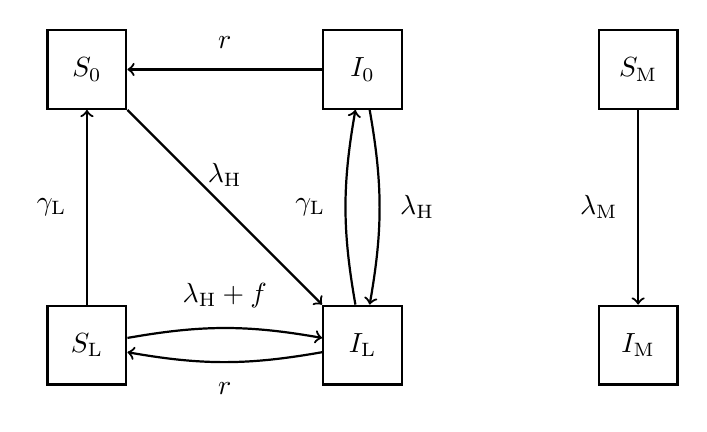
\begin{tikzpicture}[thick]
        \node[draw, minimum size=1cm] (S0) {$S_0$};
        \node[draw, right of=S0, minimum size=1cm, node distance=3.5cm] (I0)
        {$I_0$};
        \node[draw, below of=S0, minimum size=1cm, node distance=3.5cm] (SL)
        {$S_\mathrm{L}$};
        \node[draw, below of=I0, minimum size=1cm, node distance=3.5cm] (IL)
        {$I_\mathrm{L}$};
        \node[draw, right of=I0, minimum size=1cm, node distance=3.5cm] (SM)
        {$S_\mathrm{M}$};
        \node[draw, right of=IL, minimum size=1cm, node distance=3.5cm] (IM)
        {$I_\mathrm{M}$};
        \draw[->] (S0) edge node [midway, label=above:{$\lambda_\mathrm{H}$}]
        (lambdaH1) {} (IL);
        \draw[->] (SL) edge node [midway, label=left:{$\gamma_\mathrm{L}$}]
        (gammaL1) {} (S0);
        \draw[->] (SL) edge[in = 170, out = 10] node
        [midway, label=above:{$\lambda_\mathrm{H} + f$}] (lambdaf) {} (IL);
        \draw[->] (IL) edge[in = -10, out = 190] node
        [midway, label=below:{$r$}] (r) {} (SL);
        \draw[->] (IL) edge[in = 260, out = 100] node
        [midway, label=left:{$\gamma_\mathrm{L}$}] (gammaL2) {} (I0);
        \draw[->] (I0) edge[in = 80, out = 280] node
        [midway, label=right:{$\lambda_\mathrm{H}$}] (lambdaH2) {} (IL);
        \draw[->] (I0) edge node [midway, label=above:{$r$}] (r2) {} (S0);
        \draw[->] (SM) edge node [midway, label=left:{$\lambda_\mathrm{M}$}]
        (lambdaM) {} (IM);
    \end{tikzpicture}
    \caption[{
        \Citeauthor{white_variation_2016} \textit{P. vivax} model schematic
    }]{
        Diagram for \textit{P.\ vivax} model in a tropical setting described by
        \cite{white_variation_2016}. $S$ and $I$ are the number of susceptible
        and infected humans and mosquitos (denoted by subscript M).
        $\lambda_\mathrm{H} = mabI_\mathrm{M}$ and
        $\lambda_\mathrm{M} = ac(I_0 + I_\mathrm{L})$
    }
    \label{fig:white_2}
\end{figure}

One model incorporating a dormant stage is the White model
for \textit{P. vivax} depicted in
Figure \ref{fig:white_2} \parencite[Tropical Model]{white_variation_2016}.
The model is comprised of six compartments: \begin{enumerate}
    \item \textbf{
              $S_0$ (Susceptible Individuals - No Latent Hypnozoite 
              Liver-Stage Infection)
          }: People in this compartment have no form of malarial infection.
          They are susceptible to new malarial infections
          and are infected into compartment $I_\mathrm{L}$ (with both blood
          and liver-stage parasites) at rate $\lambda_\mathrm{H}$.
    \item \textbf{
              $I_\mathrm{L}$ (Infected Individuals - Both Blood-Stage and Latent
              Hypnozoite Liver-Stage Infection)
          }:  Individuals in this compartment have both an active blood-stage
          infection, and a latent hypnozoite infection in the liver.
          Individuals in $I_\mathrm{L}$ can
          progress to either $I_0$ through the clearance of liver-stage
          infection with rate $\gamma_\mathrm{L},$ or to $S_\mathrm{L}$ through
          clearance of blood-stage infection with rate $r$.
    \item \textbf{
              $I_0$ (Infected Individuals - Blood-Stage Infection Only)
          }: Individuals in $I_0$ have a blood-stage infection with no
          latent hypnozoite infection in the liver. They are be reinfected into
          $I_\mathrm{L}$ with rate $\lambda_\mathrm{H}$ and relapse with rate $f$.
          The blood-stage infection is cleared (moving into compartment $S_0$) with
          rate $r$.
    \item \textbf{
              $S_\mathrm{L}$ (Susceptible Individuals -
              Blood-Stage Infection Only)
          }: Individuals in $S_\mathrm{L}$ have latent hypnozoite infection in
          the liver without blood-stage infection. They get novel infection
          through a mosquito bite into $I_\mathrm{L}$ with rate
          $\lambda_\mathrm{H}$ or hypnozoite activation with rate $f$.
          This means those in $S_\mathrm{L}$ move to compartment
          $I_\mathrm{L}$ with a total rate $\lambda_\mathrm{H} + f.$
          Alternatively, the hypnozoites are cleared from the liver
          (moving to compartment $S_0$) with rate $\gamma_\mathrm{L}.$
    \item \textbf{
              $S_\mathrm{M}$ (Susceptible Mosquitoes)
          }:
          Suspectable mosquitoes become infectious at rate
          $\lambda_\mathrm{M}p.$ They die at rate
          $g + \lambda_\mathrm{M}(1 - p).$ Since there is a constant mosquito
          population assumption, mosquitoes are born into this state at rate
          $g + \lambda_\mathrm{M}.$
    \item \textbf{$I_\mathrm{M}$ (Infectious Mosquitoes)}:
          Infectious mosquitos die at rate $g + \lambda_\mathrm{M}(1 - p).$
\end{enumerate}

The White model is characterised by the following
ODEs:
\begin{align*}
    \frac{\diff S_0}{\diff t}
    = & -\lambda_\mathrm{H} S_0 + rI_0 + \gamma_\mathrm{L}S_\mathrm{L} \\
    \frac{\diff I_0}{\diff t}
    = & -\lambda_\mathrm{H} I_0 - rI_0 + \gamma_\mathrm{L}I_\mathrm{L} \\
    \frac{\diff S_\mathrm{L}}{\diff t}
    = & -\lambda_\mathrm{H} S_\mathrm{L} + rI_\mathrm{L}
    - fS_\mathrm{L} -\gamma_\mathrm{L}S_\mathrm{L}                     \\
    \frac{\diff I_\mathrm{L}}{\diff t}
    = & \lambda_\mathrm{H} (S_0 + I_0 + S_\mathrm{L}) - rI_\mathrm{L}
    + fS_\mathrm{L} -\gamma_\mathrm{L}I_\mathrm{L}                     \\
    \frac{\diff S_\mathrm{M}}{\diff t}
    = & g - \lambda_\mathrm{M}(pS_\mathrm{M}
    - (1 - p)I_\mathrm{M}) - gS_\mathrm{M}                             \\
    \frac{\diff I_\mathrm{M}}{\diff t}
    = & \lambda_\mathrm{M}(pS_\mathrm{M} - (1 - p)I_\mathrm{M})
    - gI_\mathrm{M}
    \tag{$I_0 + I_\mathrm{L}=$ total number of blood-stage infections}.
\end{align*}

In this model, each compartment is expressed as a proportion of the population.

The force of infection for humans is defined as
$\lambda_\mathrm{H} := mabI_\mathrm{M}$ where $m$ is the number of mosquitos
per human (held constant since there is no birth or death in the human
dynamics), $a$ is the mosquito biting rate, and $b$ is the probability that a
human bitten by an infectious mosquito develops an infection.

The force of infection for mosquitos is defined as
$\lambda_\mathrm{M} := ac(I_0 + I_\mathrm{L})$ where $a$ is defined above,
and $c$ is the probability that a mosquito bite on an infectious mosquito
causes the mosquito to become infectious. $g$ can be interpreted as the natural
birth/death rate for mosquitos. $p$ is the proportion of mosquitos that
survive long enough after the initial infection, so the parasite matures
enough in the mosquito that it can again be transmitted to humans.
Under the assumption that the time until parasite transmissibility after
infection in a mosquito is a constant of $n$ days and that mosquitoes naturally
die at rate $g$, then $p=e^{-gn}.$ To see this, let $V\sim\mathrm{Exp}(g)$
represent the mosquito's lifespan.
$\Pr(V > n)= 1 - F_V(n) = 1 - (1 - e^{-gn}) = e^{-gn}.$

$\lambda_\mathrm{M}(1 - p)$ can be interpreted as an additional rate of death,
where of the mosquitos that would develop malaria after a bite, a proportion
$1 - p$ die instantly. This applies to both the susceptible and infectious
mosquitoes. Presumably, this approximates a model where mosquitoes are moved
to an `exposed' compartment for $n$ time, after initial infection.
However, no justification is given by \Citeauthor{white_variation_2016} for
this additional parameter $n$. A more straightforward $SI$ model could be
constructed that absorbs $c$ and $n$ into the single parameter $c^*$, such
that it becomes the proportion of mosquito bites on blood-stage infectious
humans that result in mosquito infection where the mosquito does not die
before becoming infectious. With a steady mosquito population, the mosquito
dynamics would now be characterised by
$$
    \frac{\diff I_\mathrm{M}}{\diff t}
    = \lambda_\mathrm{M}^*S_\mathrm{M} - gI_\mathrm{M}
    \quad\text{where } \lambda_\mathrm{M}^*:= ac^*(I_0 + I_\mathrm{L}).
$$

By modelling both liver-stage and blood-stage infection, blood-stage infections
from relapses can be captured in the dynamics, meaning it is possible to
analyse case number data that may be confounded by relapses as well as
novel infections.

This model does not account for continual depletion of liver-stage parasites,
which would vary the rate of relapse over time (through clearance or relapse).
It also does not directly model any interventions or case importations. The
lack of population dynamics means the model may only be useful on a small time
scale. Finally, it does not account for any importation of disease from an
outside area, so if $S_0 = 1,$ \textit{P.\ vivax} is presumed permanently
eradicated.

\subsubsection*{Champagne Model}\label{sec:champ_mod}

\begin{figure}[htbp]
    \centering
    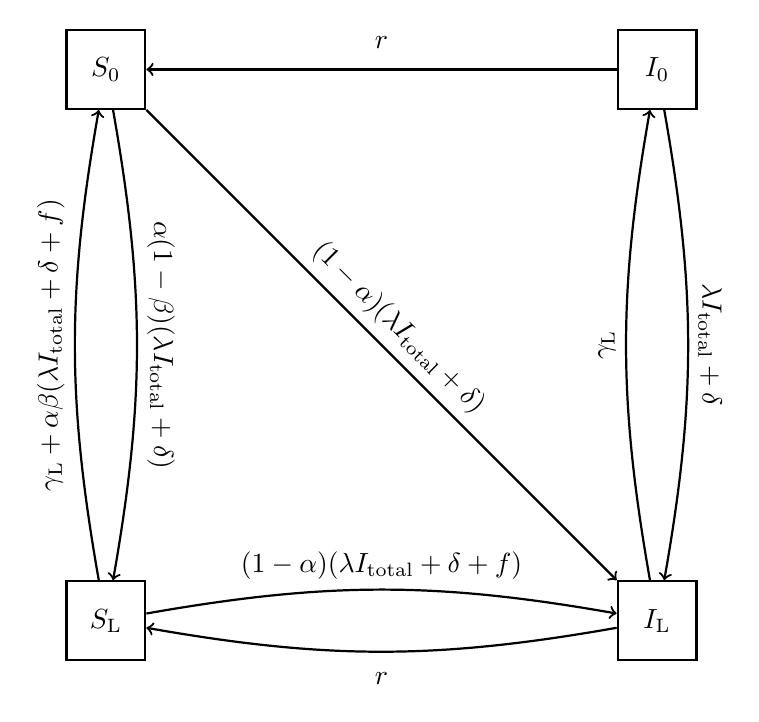
\begin{tikzpicture}[thick]
        \node[draw, minimum size=1cm] (S0) {$S_0$};
        \node[draw, right of=S0, minimum size=1cm, node distance=7cm] (I0) {$I_0$};
        \node[draw, below of=S0, minimum size=1cm, node distance=7cm] (SL) {$S_\mathrm{L}$};
        \node[draw, below of=I0, minimum size=1cm, node distance=7cm] (IL) {$I_\mathrm{L}$};
        \draw[->] (S0) edge[sloped] node[above] {$(1 - \alpha)(\lambda I_\mathrm{total} + \delta)$} (IL);
        \draw[->] (S0) edge[in = 80, out = 280, sloped] node[above] {$\alpha( 1 -\beta)(\lambda I_\mathrm{total} + \delta)$} (SL);
        \draw[->] (SL) edge[in = 260, out = 100, sloped] node [above] {$\gamma_\mathrm{L} + \alpha\beta(\lambda I_\mathrm{total} + \delta + f)$} (S0);
        \draw[->] (SL) edge[in = 170, out = 10, sloped] node [above] {$(1 -\alpha)(\lambda I_\mathrm{total} + \delta + f)$} (IL);
        \draw[->] (IL) edge[in = -10, out = 190] node [midway, label=below:{$r$}] (r) {} (SL);
        \draw[->] (IL) edge[in = 260, out = 100, sloped] node [above] {$\gamma_\mathrm{L}$} (I0);
        \draw[->] (I0) edge[in = 80, out = 280, sloped] node [above] {$\lambda I_\mathrm{total} + \delta$} (IL);
        \draw[->] (I0) edge node [midway, label=above:{$r$}] (r2) {} (S0);
    \end{tikzpicture}
    \caption[{
        \Citeauthor{champagne_using_2022} \textit{P. vivax} model schematic
    }]{
        Diagram for \textit{P.\ vivax} model described by
        \cite{champagne_using_2022}.
        $I_\mathrm{total} = I_0 + I _\mathrm{L}.$ Since the mosquito dynamics
        have been removed, $\lambda$ now has no dependencies on the number
        of infectious mosquitos.
    }
    \label{fig:champ_diag}
\end{figure}

The Champagne model - described in \parencite{champagne_using_2022} and
diagrammatically depicted in Figure \ref{fig:champ_diag} -
simultaneously simplifies and extends the White model. The model assumes 
human-to-human 
transmission, removing mosquito dynamics, and extends it by adding
in a rate of imported cases and treatment of malarial infection.
It is characterised by the system of ODEs:
\begin{align*}
    \frac{\diff I_\mathrm{L}}{\diff t}
    = & (1 - \alpha)(\lambda I_\mathrm{total} + \delta)(S_0 + S_\mathrm{L})
    + (\lambda I_\mathrm{total} + \delta)I_0 + (1 - \alpha)fS_\mathrm{L}
    - \gamma_\mathrm{L}I_\mathrm{L} - rI_\mathrm{L}                         \\
    \frac{\diff I_0}{\diff t}
    = & -(\lambda I_\mathrm{total} + \delta)I_0
    + \gamma_\mathrm{L}I_\mathrm{L} - rI_0                                  \\
    \frac{\diff S_\mathrm{L}}{\diff t}
    = & -(1 - \alpha(1 - \beta))(\lambda I_\mathrm{total} + \delta + f)
    S_\mathrm{L} + \alpha(1-\beta)(\lambda I_\mathrm{total} + \delta)S_0
    - \gamma_\mathrm{L}S_\mathrm{L} + rI_\mathrm{L}                         \\
    \frac{\diff S_0}{\diff t}
    = & -(1 - \alpha\beta)(\lambda I_\mathrm{total} + \delta)S_0
    + (\lambda I_\mathrm{total} + \delta)\alpha\beta S_\mathrm{L}
    + \alpha\beta fS_\mathrm{L} + \gamma_\mathrm{L}S_\mathrm{L} + rI_0,
\end{align*} where $I_\mathrm{total} := I_0 + I_\mathrm{L}.$

The compartments $S_0, I_0, I_\mathrm{L}$ and $S_\mathrm{L}$
have the same interpretation as in the White model,
however the rates between compartments are significantly modified.

The new parameters are
\begin{itemize}
    \item $\lambda:$ the rate of infection
    \item $\delta:$ importation rate
    \item $\alpha:$ proportion of those infected who clear blood-stage
          infections through immediate treatment, and
    \item $\beta:$ proportion of those cleared of blood-stage infection who
          are also cleared of liver-stage parasites (radical cure).
\end{itemize}
In other words, the proportion $\alpha\beta$ of infected individuals is
wholly cured of liver-stage and blood-stage parasites. The model assumes
treatment clears the infection instantaneously. Individuals in $S_\mathrm{L}$ who
relapse or get a new infection are assumed to be cured with the same
proportions as new infections from $S_0.$ However, individuals in $I_0$ who are
superinfected are assumed not to seek treatment.

In contrast to the White model, the Champagne model allows analysis of
potential treatment interventions or how much of an impact limiting the
importation rate might have on case numbers (through border control/testing).
Although the lack of mosquito dynamics simplifies the model and it's running,
it is unrealistic. The model still has some of the same problems as the White
model, such as not incorporating hypnozoite depletion rates and a lack of
population dynamics, meaning all analytic results are done assuming the system
is at equilibrium.